\documentclass[10pt, notes, handout]{beamer}

\usepackage[utf8x]{inputenc}
\usepackage[T1]{fontenc}
\usepackage{lmodern}
\usepackage{microtype}
\usepackage{xspace}
%\usepackage[binary-units=true]{siunitx}
\usepackage{graphicx}
\usepackage{hyperref}
\usepackage{todonotes}
\usepackage{epstopdf}
\usepackage{array}
\usepackage{multicol}
\usepackage{multirow}
\usepackage{tabularx} 	% tabular with automatic line-break
\newcolumntype{Y}{>{\centering\arraybackslash}X} % centered column
\usepackage{amsmath}
\usepackage{grffile} 	% better name handling with graphicx
\usepackage{currfile} 	% provides relative file inclusion for tikzscale

\usepackage[]{algorithm2e}

\usepackage{tikz}
\usepackage{pgfplots}
\usepackage{tikzscale}
\pgfplotsset{compat=newest}
\usetikzlibrary{plotmarks}
\usepackage[absolute,overlay]{textpos}

% Math symbols
\usepackage{amsmath}
\usepackage{amssymb}
\usepackage{amsthm}
\DeclareMathOperator*{\argmin}{arg\,min}
\DeclareMathOperator*{\argmax}{arg\,max}
\newcommand\norm[1]{\left\lVert#1\right\rVert}

% Sets
\newcommand{\Z}{\mathbb{Z}}
\newcommand{\R}{\mathbb{R}}
\newcommand{\Rn}{\R^n}
\newcommand{\Rnn}{\R^{n \times n}}
\newcommand{\C}{\mathbb{C}}
\newcommand{\K}{\mathbb{K}}
\newcommand{\Kn}{\K^n}
\newcommand{\Knn}{\K^{n \times n}}

\newcommand\eqdef{\triangleq}

% Vectors
\newcommand{\vct}[1]{\boldsymbol{#1}}
\newcommand{\va}{\vct{a}}
\newcommand{\vb}{\vct{b}}
\newcommand{\vc}{\vct{c}}
\newcommand{\vd}{\vct{d}}
\newcommand{\ve}{\vct{e}}
\newcommand{\vf}{\vct{f}}
\newcommand{\vg}{\vct{g}}
\newcommand{\vh}{\vct{h}}
\newcommand{\vi}{\vct{i}}
\newcommand{\vj}{\vct{j}}
\newcommand{\vk}{\vct{k}}
\newcommand{\vl}{\vct{l}}
\newcommand{\vm}{\vct{m}}
\newcommand{\vn}{\vct{n}}
\newcommand{\vo}{\vct{o}}
\newcommand{\vp}{\vct{p}}
\newcommand{\vq}{\vct{q}}
\newcommand{\vr}{\vct{r}}
\newcommand{\vs}{\vct{s}}
\newcommand{\vt}{\vct{t}}
\newcommand{\vu}{\vct{u}}
\newcommand{\vv}{\vct{v}}
\newcommand{\vw}{\vct{w}}
\newcommand{\vx}{\vct{x}}
\newcommand{\vy}{\vct{y}}
\newcommand{\vz}{\vct{z}}
% Greek letter vectors
\newcommand{\valpha}{\vct{\alpha}}
\newcommand{\vbeta}{\vct{\beta}}
\newcommand{\vepsilon}{\vct{\epsilon}}
\newcommand{\vgamma}{\vct{\gamma}}
\newcommand{\vlambda}{\vct{\lambda}}
\newcommand{\vnu}{\vct{\nu}}
\newcommand{\vphi}{\vct{\phi}}
\newcommand{\vpsi}{\vct{\psi}}
\newcommand{\vtheta}{\vct{\theta}}
\newcommand{\vxi}{\vct{\xi}}
\newcommand{\vzero}{\vct{0}}
\newcommand{\vone}{\vct{1}}
% Matrices
\newcommand{\mtx}[1]{\boldsymbol{#1}}
\newcommand{\mzero}{\mtx{0}}
\newcommand{\mA}{\mtx{A}}
\newcommand{\mB}{\mtx{B}}
\newcommand{\mC}{\mtx{C}}
\newcommand{\mD}{\mtx{D}}
\newcommand{\mE}{\mtx{E}}
\newcommand{\mF}{\mtx{F}}
\newcommand{\mG}{\mtx{G}}
\newcommand{\mH}{\mtx{H}}
\newcommand{\mI}{\mtx{I}}
\newcommand{\mJ}{\mtx{J}}
\newcommand{\mK}{\mtx{K}}
\newcommand{\mL}{\mtx{L}}
\newcommand{\mM}{\mtx{M}}
\newcommand{\mN}{\mtx{N}}
\newcommand{\mO}{\mtx{O}}
\newcommand{\mP}{\mtx{P}}
\newcommand{\mQ}{\mtx{Q}}
\newcommand{\mR}{\mtx{R}}
\newcommand{\mS}{\mtx{S}}
\newcommand{\mT}{\mtx{T}}
\newcommand{\mU}{\mtx{U}}
\newcommand{\mV}{\mtx{V}}
\newcommand{\mW}{\mtx{W}}
\newcommand{\mX}{\mtx{X}}
\newcommand{\mY}{\mtx{Y}}
\newcommand{\mZ}{\mtx{Z}}

\usepackage{comment}
\usepackage{pgfpages}
\usepackage{bm}

\usetheme[progressbar=frametitle]{metropolis}
\tikzset{font={\fontsize{10pt}{12}\selectfont}}
\usepackage{hf-tikz}
\usetikzlibrary{ 
	calc,
	arrows,
	arrows.meta,
	automata, 
	shapes, 
	snakes, 
	positioning, 
	decorations,
	decorations.text,
	fit,
	matrix,
	mindmap
	}
\tikzstyle{noeud-std}=[draw,fill=black,circle,inner sep=0pt,minimum size=7pt]
\usepackage{tkz-graph}
\usepackage{xspace}
\usepackage{amsmath}
\usepackage{mathtools}

\definecolor{green}{HTML}{14B03D}
\newcommand{\payoff}[2]{{\color{green}#1}, {\color{red}#2}}

\usepackage{comment}
\usepackage{pgfpages}
\usepackage{bm}

\usetheme[progressbar=frametitle]{metropolis}
\tikzset{font={\fontsize{10pt}{12}\selectfont}}
\usepackage{hf-tikz}
\usetikzlibrary{ 
	calc,
	arrows,
	arrows.meta,
	automata, 
	shapes, 
	snakes, 
	positioning, 
	decorations,
	decorations.text,
	fit,
	matrix,
	mindmap
	}
	\tikzstyle{noeud-std}=[draw,fill=black,circle,inner sep=0pt,minimum size=7pt]% 7pt est la taille des cercles noirs
\usepackage{tkz-graph}
\newcommand{\tikzmark}[2]{\tikz[overlay,remember picture,baseline=(#1.base)] \node (#1) {#2};}
\newcommand{\Highlight}[1][submatrix]{%
    \tikz[overlay,remember picture]{
    \node[highlight,fit=(left.north west) (right.south east)] (#1) {};}
    }
\tikzset{%
  highlight/.style={rectangle,rounded corners,fill=ocre!50,draw,
    fill opacity=0.5,thick,inner sep=0pt}
}
\newcommand{\mytikzmark}[2]{\tikz[overlay,remember picture, baseline=(#1.base)] \node (#1) {#2};}

\usepackage{xspace}
\usepackage{amsmath}
\usepackage{mathtools}

%[doi=false,isbn=false,note=false,url=false,eprint=false, backend=bibtex]
\usepackage{biblatex} 
%\AtEveryCitekey{\clearfield{note}\clearlist{location}\clearlist{publisher}\clearname{editor}}
%\bibliographystyle{plain}
\bibliography{biblio}

\definecolor{green}{HTML}{14B03D}
\newcommand{\payoff}[2]{{\color{green}#1}, {\color{red}#2}}

\title{LINMA2345 - Game theory}
\subtitle{Repeated games}
\date{\today}
\author{Antoine Gennart\and Jonathan Sarteel\and Antoine Paris}
\institute{Ecole polytechnique de Louvain}
\titlegraphic{\hfill
\includegraphics[height=1cm]{logo}}

\begin{document}
\maketitle

\begin{frame}{Outline}
    \setbeamertemplate{sections in toc}[sections numbered]
    \tableofcontents[hideallsubsections]
\end{frame}

\begin{frame}{Outline}
    \tableofcontents[currentsection]
\end{frame}

\section{Finitely repeated games}
\begin{frame}{What is a finitely repeated games?}
    In a \textit{finitely repeated game}, players
    \begin{itemize}
        \item play the same game for a finite number of times $K$,
        \textbf{known by the players before the game starts}, and
        \item collect their payoffs after each round (and thus observe what
        the others played).
    \end{itemize}

    \begin{figure}[!ht]
        \centering
        \begin{tikzpicture}[->,>=stealth',shorten >=1pt,auto,node distance=2cm, semithick, scale = 1,
            transform shape ]
            \node	        (start)								{Start};
            \node[state] 	(n1)    	[right of = start]		{Round 1};
            \node[state] 	(n2)		[right of = n1]			{Round 2};
            \node	        (dots)		[right of = n2]			{$\cdots$};
            \node[state] 	(nk)		[right of = dots]		{Round $K$};
            \node	        (stop)		[right of = nk]			{Stop};
            \path 	(start) edge node {}	(n1)
                    (n1)	edge node {}	(n2)
                    (n2)	edge node {}	(dots)
                    (dots)	edge node {}	(nk)
                    (nk) 	edge node {}	(stop);
        \end{tikzpicture}
        \caption{Finitely Repeated Games.}
    \end{figure}
\end{frame}

\begin{frame}{Let's play the Prisoner's Dilemma 2 times}
    \begin{exampleblock}{Example}
        Consider the Prisoner's Dilemma in normal form.
        \begin{table}
            \begin{tabular}{c|cc}
                & {\color{red}c}    & {\color{red}d} \\
                \hline
                {\color{green}C}    & \payoff{-1}{-1}   & \payoff{-4}{~0} \\
                {\color{green}D}    & \payoff{~0}{-4}    & \payoff{-3}{-3} 
            \end{tabular}
            \caption{Prisoner's Dilemma in normal form.}
        \end{table}
    
        \begin{itemize}
            \item The only Nash Equilibrium of this game is for both
            players to defect.
            \item Let's play this game 2 times in a row and see what happens.
        \end{itemize}
        
        \vspace{0.5cm}
        \hfill \textit{Hint}: \reflectbox{think backward}.

    \end{exampleblock}
\end{frame}

\note{
    Draw a table on the blackboard and collect the actions/outcomes of each pair
    of students after each round.

    At the end, quickly compare the result. Ask students to motivate their strategy
    choice (especially if it differs from what a rationnal player would do).

    Probably the audience will cooperate more than expected.
}

\begin{frame}{The twice repeated Prisoner's Dilemma: Nash Equilibrium}
We proceed by \textit{backward induction} to find the Nash Equilibrium.
\begin{figure}[!ht]
    \centering
    \scalebox{0.65}{
    \begin{tikzpicture}
    \node[noeud-std, color=green] (n1) {}
       [sibling distance=8cm]
          child {node[noeud-std, color=red] (n2-1c) {} % 1
          [sibling distance=4cm]
                 child{node[noeud-std, color=green] (n1-1c2c){} % 2
                    [sibling distance=2cm]
                    child{node[noeud-std, color=red] (n2-1c2c1c){}  % 1
                        [sibling distance = 1cm]
                             child[level distance=1.5cm]{node[noeud-std,fill=white] (p-1c2c1c2c){} } % 1
                             child[level distance=2.5cm]{node[noeud-std,fill=white] (p-1c2c1c2d){} } % 1
                         }
                    child{node[noeud-std, color=red] (n2-1c2c1d){}  % 1
                        [sibling distance = 1cm]
                            child[level distance=1.5cm]{node[noeud-std,fill=white] (p-1c2c1d2c){} } % 1
                            child[level distance=2.5cm]{node[noeud-std,fill=white] (p-1c2c1d2d){} } % 1
                        }
                }
                child{node[noeud-std, color=green] (n1-1c2d){} % 2
                    [sibling distance=2cm]
                    child{node[noeud-std, color=red] (n2-1c2d1c){}  % 1
                        [sibling distance = 1cm]
                             child[level distance=1.5cm]{node[noeud-std,fill=white] (p-1c2d1c2c){} } % 1
                             child[level distance=2.5cm]{node[noeud-std,fill=white] (p-1c2d1c2d){} } % 1
                         }
                    child{node[noeud-std, color=red] (n2-1c2d1d){}  % 1
                        [sibling distance = 1cm]
                            child[level distance=1.5cm]{node[noeud-std,fill=white] (p-1c2d1d2c){} } % 1
                            child[level distance=2.5cm]{node[noeud-std,fill=white] (p-1c2d1d2d){} } % 1
                        }
                }
       }
       child {node[noeud-std, color=red] (n2-1d) {} % 1
          [sibling distance=4cm]
                 child{node[noeud-std, color=green] (n1-1d2c){} % 2
                    [sibling distance=2cm]
                    child{node[noeud-std, color=red] (n2-1d2c1c){}  % 1
                        [sibling distance = 1cm]
                             child[level distance=1.5cm]{node[noeud-std,fill=white] (p-1d2c1c2c){} } % 1
                             child[level distance=2.5cm]{node[noeud-std,fill=white] (p-1d2c1c2d){} } % 1
                         }
                    child{node[noeud-std, color=red] (n2-1d2c1d){}  % 1
                        [sibling distance = 1cm]
                            child[level distance=1.5cm]{node[noeud-std,fill=white] (p-1d2c1d2c){} } % 1
                            child[level distance=2.5cm]{node[noeud-std,fill=white] (p-1d2c1d2d){} } % 1
                        }
                }
                child{node[noeud-std, color=green] (n1-1d2d){} % 2
                    [sibling distance=2cm]
                    child{node[noeud-std, color=red] (n2-1d2d1c){}  % 1
                        [sibling distance = 1cm]
                             child[level distance=1.5cm]{node[noeud-std,fill=white] (p-1d2d1c2c){} } % 1
                             child[level distance=2.5cm]{node[noeud-std,fill=white] (p-1d2d1c2d){} } % 1
                         }
                    child{node[noeud-std, color=red] (n2-1d2d1d){}  % 1
                        [sibling distance = 1cm]
                            child[level distance=1.5cm]{node[noeud-std,fill=white] (p-1d2d1d2c){} } % 1
                            child[level distance=2.5cm]{node[noeud-std,fill=white] (p-1d2d1d2d){} } % 1
                        }
                }
       }

    ;
    %
    \node[above=5pt] at (n1) {1.a};
    \node[above left] at ($(n1)!{0.5}!(n2-1c)$) {C};
    \node[above right] at ($(n1)!{0.5}!(n2-1d)$) {D};

    \node[above=5pt] at (n2-1c) {2.b};
    \node[above left] at ($(n2-1c)!{0.5}!(n1-1c2c)$) {c};
    \node[above right] at ($(n2-1c)!{0.5}!(n1-1c2d)$) {d};
    \node[above=5pt] at (n1-1c2c) {1.c};
    \node[above left] at ($(n1-1c2c)!{0.5}!(n2-1c2c1c)$) {C};
    \node[above right] at ($(n1-1c2c)!{0.5}!(n2-1c2c1d)$) {D};
    \node[above=5pt] at (n2-1c2c1d) {2.d};
    \node[above left] at ($(n2-1c2c1d)!{0.5}!(p-1c2c1d2c)$) {c};
    \node[above right] at ($(n2-1c2c1d)!{0.5}!(p-1c2c1d2d)$) {d};
    \node[above=5pt] at (n2-1c2c1c) {2.d};
    \node[above left] at ($(n2-1c2c1c)!{0.5}!(p-1c2c1c2c)$) {c};
    \node[above right] at ($(n2-1c2c1c)!{0.5}!(p-1c2c1c2d)$) {d};
    \node[above=5pt] at (n1-1c2d) {1.e};
    \node[above left] at ($(n1-1c2d)!{0.5}!(n2-1c2d1c)$) {C};
    \node[above right] at ($(n1-1c2d)!{0.5}!(n2-1c2d1d)$) {D};
    \node[above=5pt] at (n2-1c2d1d) {2.f};
    \node[above left] at ($(n2-1c2d1d)!{0.5}!(p-1c2d1d2c)$) {c};
    \node[above right] at ($(n2-1c2d1d)!{0.5}!(p-1c2d1d2d)$) {d};
    \node[above=5pt] at (n2-1c2d1c) {2.f};
    \node[above left] at ($(n2-1c2d1c)!{0.5}!(p-1c2d1c2c)$) {c};
    \node[above right] at ($(n2-1c2d1c)!{0.5}!(p-1c2d1c2d)$) {d};

    \node[above=5pt] at (n2-1d) {2.b};
    \node[above left] at ($(n2-1d)!{0.5}!(n1-1d2c)$) {c};
    \node[above right] at ($(n2-1d)!{0.5}!(n1-1d2d)$) {d};
    \node[above=5pt] at (n1-1d2c) {1.g};
    \node[above left] at ($(n1-1d2c)!{0.5}!(n2-1d2c1c)$) {C};
    \node[above right] at ($(n1-1d2c)!{0.5}!(n2-1d2c1d)$) {D};
    \node[above=5pt] at (n2-1d2c1d) {2.h};
    \node[above left] at ($(n2-1d2c1d)!{0.5}!(p-1d2c1d2c)$) {c};
    \node[above right] at ($(n2-1d2c1d)!{0.5}!(p-1d2c1d2d)$) {d};
    \node[above=5pt] at (n2-1d2c1c) {2.h};
    \node[above left] at ($(n2-1d2c1c)!{0.5}!(p-1d2c1c2c)$) {c};
    \node[above right] at ($(n2-1d2c1c)!{0.5}!(p-1d2c1c2d)$) {d};
    \node[above=5pt] at (n1-1d2d) {1.i};
    \node[above left] at ($(n1-1d2d)!{0.5}!(n2-1d2d1c)$) {C};
    \node[above right] at ($(n1-1d2d)!{0.5}!(n2-1d2d1d)$) {D};
    \node[above=5pt] at (n2-1d2d1d) {2.j};
    \node[above left] at ($(n2-1d2d1d)!{0.5}!(p-1d2d1d2c)$) {c};
    \node[above right] at ($(n2-1d2d1d)!{0.5}!(p-1d2d1d2d)$) {d};
    \node[above=5pt] at (n2-1d2d1c) {2.j};
    \node[above left] at ($(n2-1d2d1c)!{0.5}!(p-1d2d1c2c)$) {c};
    \node[above right] at ($(n2-1d2d1c)!{0.5}!(p-1d2d1c2d)$) {d};

    \path (n2-1d)  edge [dashed] node {} (n2-1c);
    \path (n2-1c2c1d)  edge [dashed] node {} (n2-1c2c1c);
    \path (n2-1c2d1d)  edge [dashed] node {} (n2-1c2d1c);
    \path (n2-1d2c1d)  edge [dashed] node {} (n2-1d2c1c);
    \path (n2-1d2d1d)  edge [dashed] node {} (n2-1d2d1c);

    \node[below = 5pt] at ($(p-1c2c1c2c)$) {\payoff{-2}{-2}};
    \node[below = 5pt] at ($(p-1c2c1c2d)$) {\payoff{-5}{-1}};
    \node[below = 5pt] at ($(p-1c2c1d2c)$) {\payoff{-1}{-5}};
    \node[below = 5pt] at ($(p-1c2c1d2d)$) {\payoff{-4}{-4}};


    \node[below = 5pt] at ($(p-1c2d1c2c)$) {\payoff{-5}{-1}};
    \node[below = 5pt] at ($(p-1c2d1c2d)$) {\payoff{-8}{0}};
    \node[below = 5pt] at ($(p-1c2d1d2c)$) {\payoff{-4}{-4}};
    \node[below = 5pt] at ($(p-1c2d1d2d)$) {\payoff{-7}{-3}};


    \node[below = 5pt] at ($(p-1d2c1c2c)$) {\payoff{-1}{-5}};
    \node[below = 5pt] at ($(p-1d2c1c2d)$) {\payoff{-4}{-4}};
    \node[below = 5pt] at ($(p-1d2c1d2c)$) {\payoff{0}{-8}};
    \node[below = 5pt] at ($(p-1d2c1d2d)$) {\payoff{-3}{-7}};


    \node[below = 5pt] at ($(p-1d2d1c2c)$) {\payoff{-4}{-4}};
    \node[below = 5pt] at ($(p-1d2d1c2d)$) {\payoff{-7}{-3}};
    \node[below = 5pt] at ($(p-1d2d1d2c)$) {\payoff{-3}{-7}};
    \node[below = 5pt] at ($(p-1d2d1d2d)$) {\payoff{-6}{-6}};

    \end{tikzpicture}}
    \caption{Prisoner's Dilemma repeated twice in extensive form.}
\end{figure}

\end{frame}

\begin{frame}{Nash equilibrium: backward induction (1)}
\begin{figure}[!ht]
\centering
\scalebox{0.65}{
\begin{tikzpicture}
\node[noeud-std, color=green] (n1) {}
   [sibling distance=8cm]
      child {node[noeud-std, color=red] (n2-1c) {} % 1
      [sibling distance=4cm]
             child{node[noeud-std, color=green] (n1-1c2c){} % 2
                [sibling distance=2cm]
                child{node[noeud-std, color=red] (n2-1c2c1c){}  % 1
                    [sibling distance = 1cm]
                         child[level distance=1.5cm]{node[noeud-std,fill=white] (p-1c2c1c2c){} } % 1
                         child[level distance=2.5cm, very thick, red]{node[noeud-std,fill=white] (p-1c2c1c2d){} } % 1
                     }
                child{node[noeud-std, color=red] (n2-1c2c1d){}  % 1
                    [sibling distance = 1cm]
                        child[level distance=1.5cm]{node[noeud-std,fill=white] (p-1c2c1d2c){} } % 1
                        child[level distance=2.5cm, very thick, red]{node[noeud-std,fill=white] (p-1c2c1d2d){} } % 1
                    }
            }
            child{node[noeud-std, color=green] (n1-1c2d){} % 2
                [sibling distance=2cm]
                child{node[noeud-std, color=red] (n2-1c2d1c){}  % 1
                    [sibling distance = 1cm]
                         child[level distance=1.5cm]{node[noeud-std,fill=white] (p-1c2d1c2c){} } % 1
                         child[level distance=2.5cm, very thick, red]{node[noeud-std,fill=white] (p-1c2d1c2d){} } % 1
                     }
                child{node[noeud-std, color=red] (n2-1c2d1d){}  % 1
                    [sibling distance = 1cm]
                        child[level distance=1.5cm]{node[noeud-std,fill=white] (p-1c2d1d2c){} } % 1
                        child[level distance=2.5cm, very thick, red]{node[noeud-std,fill=white] (p-1c2d1d2d){} } % 1
                    }
            }
   }
   child {node[noeud-std, color=red] (n2-1d) {} % 1
      [sibling distance=4cm]
             child{node[noeud-std, color=green] (n1-1d2c){} % 2
                [sibling distance=2cm]
                child{node[noeud-std, color=red] (n2-1d2c1c){}  % 1
                    [sibling distance = 1cm]
                         child[level distance=1.5cm]{node[noeud-std,fill=white] (p-1d2c1c2c){} } % 1
                         child[level distance=2.5cm, very thick, red]{node[noeud-std,fill=white] (p-1d2c1c2d){} } % 1
                     }
                child{node[noeud-std, color=red] (n2-1d2c1d){}  % 1
                    [sibling distance = 1cm]
                        child[level distance=1.5cm]{node[noeud-std,fill=white] (p-1d2c1d2c){} } % 1
                        child[level distance=2.5cm, very thick, red]{node[noeud-std,fill=white] (p-1d2c1d2d){} } % 1
                    }
            }
            child{node[noeud-std, color=green] (n1-1d2d){} % 2
                [sibling distance=2cm]
                child{node[noeud-std, color=red] (n2-1d2d1c){}  % 1
                    [sibling distance = 1cm]
                         child[level distance=1.5cm]{node[noeud-std,fill=white] (p-1d2d1c2c){} } % 1
                         child[level distance=2.5cm, very thick, red]{node[noeud-std,fill=white] (p-1d2d1c2d){} } % 1
                     }
                child{node[noeud-std, color=red] (n2-1d2d1d){}  % 1
                    [sibling distance = 1cm]
                        child[level distance=1.5cm]{node[noeud-std,fill=white] (p-1d2d1d2c){} } % 1
                        child[level distance=2.5cm, very thick, red]{node[noeud-std,fill=white] (p-1d2d1d2d){} } % 1
                    }
            }
   }

;
%
\node[above=5pt] at (n1) {1.a};
\node[above left] at ($(n1)!{0.5}!(n2-1c)$) {C};
\node[above right] at ($(n1)!{0.5}!(n2-1d)$) {D};

\node[above=5pt] at (n2-1c) {2.b};
\node[above left] at ($(n2-1c)!{0.5}!(n1-1c2c)$) {c};
\node[above right] at ($(n2-1c)!{0.5}!(n1-1c2d)$) {d};
\node[above=5pt] at (n1-1c2c) {1.c};
\node[above left] at ($(n1-1c2c)!{0.5}!(n2-1c2c1c)$) {C};
\node[above right] at ($(n1-1c2c)!{0.5}!(n2-1c2c1d)$) {D};
\node[above=5pt] at (n2-1c2c1d) {2.d};
\node[above left] at ($(n2-1c2c1d)!{0.5}!(p-1c2c1d2c)$) {c};
\node[above right] at ($(n2-1c2c1d)!{0.5}!(p-1c2c1d2d)$) {d};
\node[above=5pt] at (n2-1c2c1c) {2.d};
\node[above left] at ($(n2-1c2c1c)!{0.5}!(p-1c2c1c2c)$) {c};
\node[above right] at ($(n2-1c2c1c)!{0.5}!(p-1c2c1c2d)$) {d};
\node[above=5pt] at (n1-1c2d) {1.e};
\node[above left] at ($(n1-1c2d)!{0.5}!(n2-1c2d1c)$) {C};
\node[above right] at ($(n1-1c2d)!{0.5}!(n2-1c2d1d)$) {D};
\node[above=5pt] at (n2-1c2d1d) {2.f};
\node[above left] at ($(n2-1c2d1d)!{0.5}!(p-1c2d1d2c)$) {c};
\node[above right] at ($(n2-1c2d1d)!{0.5}!(p-1c2d1d2d)$) {d};
\node[above=5pt] at (n2-1c2d1c) {2.f};
\node[above left] at ($(n2-1c2d1c)!{0.5}!(p-1c2d1c2c)$) {c};
\node[above right] at ($(n2-1c2d1c)!{0.5}!(p-1c2d1c2d)$) {d};

\node[above=5pt] at (n2-1d) {2.b};
\node[above left] at ($(n2-1d)!{0.5}!(n1-1d2c)$) {c};
\node[above right] at ($(n2-1d)!{0.5}!(n1-1d2d)$) {d};
\node[above=5pt] at (n1-1d2c) {1.g};
\node[above left] at ($(n1-1d2c)!{0.5}!(n2-1d2c1c)$) {C};
\node[above right] at ($(n1-1d2c)!{0.5}!(n2-1d2c1d)$) {D};
\node[above=5pt] at (n2-1d2c1d) {2.h};
\node[above left] at ($(n2-1d2c1d)!{0.5}!(p-1d2c1d2c)$) {c};
\node[above right] at ($(n2-1d2c1d)!{0.5}!(p-1d2c1d2d)$) {d};
\node[above=5pt] at (n2-1d2c1c) {2.h};
\node[above left] at ($(n2-1d2c1c)!{0.5}!(p-1d2c1c2c)$) {c};
\node[above right] at ($(n2-1d2c1c)!{0.5}!(p-1d2c1c2d)$) {d};
\node[above=5pt] at (n1-1d2d) {1.i};
\node[above left] at ($(n1-1d2d)!{0.5}!(n2-1d2d1c)$) {C};
\node[above right] at ($(n1-1d2d)!{0.5}!(n2-1d2d1d)$) {D};
\node[above=5pt] at (n2-1d2d1d) {2.j};
\node[above left] at ($(n2-1d2d1d)!{0.5}!(p-1d2d1d2c)$) {c};
\node[above right] at ($(n2-1d2d1d)!{0.5}!(p-1d2d1d2d)$) {d};
\node[above=5pt] at (n2-1d2d1c) {2.j};
\node[above left] at ($(n2-1d2d1c)!{0.5}!(p-1d2d1c2c)$) {c};
\node[above right] at ($(n2-1d2d1c)!{0.5}!(p-1d2d1c2d)$) {d};

\path (n2-1d)  edge [dashed] node {} (n2-1c);
\path (n2-1c2c1d)  edge [dashed] node {} (n2-1c2c1c);
\path (n2-1c2d1d)  edge [dashed] node {} (n2-1c2d1c);
\path (n2-1d2c1d)  edge [dashed] node {} (n2-1d2c1c);
\path (n2-1d2d1d)  edge [dashed] node {} (n2-1d2d1c);

\node[below = 5pt] at ($(p-1c2c1c2c)$) {\payoff{-2}{-2}};
\node[below = 5pt] at ($(p-1c2c1c2d)$) {\textbf{\payoff{-5}{-1}}};
\node[below = 5pt] at ($(p-1c2c1d2c)$) {\payoff{-1}{-5}};
\node[below = 5pt] at ($(p-1c2c1d2d)$) {\textbf{\payoff{-4}{-4}}};


\node[below = 5pt] at ($(p-1c2d1c2c)$) {\payoff{-5}{-1}};
\node[below = 5pt] at ($(p-1c2d1c2d)$) {\textbf{\payoff{-8}{0}}};
\node[below = 5pt] at ($(p-1c2d1d2c)$) {\payoff{-4}{-4}};
\node[below = 5pt] at ($(p-1c2d1d2d)$) {\textbf{\payoff{-7}{-3}}};


\node[below = 5pt] at ($(p-1d2c1c2c)$) {\payoff{-1}{-5}};
\node[below = 5pt] at ($(p-1d2c1c2d)$) {\textbf{\payoff{-4}{-4}}};
\node[below = 5pt] at ($(p-1d2c1d2c)$) {\payoff{0}{-8}};
\node[below = 5pt] at ($(p-1d2c1d2d)$) {\textbf{\payoff{-3}{-7}}};


\node[below = 5pt] at ($(p-1d2d1c2c)$) {\payoff{-4}{-4}};
\node[below = 5pt] at ($(p-1d2d1c2d)$) {\textbf{\payoff{-7}{-3}}};
\node[below = 5pt] at ($(p-1d2d1d2c)$) {\payoff{-3}{-7}};
\node[below = 5pt] at ($(p-1d2d1d2d)$) {\textbf{\payoff{-6}{-6}}};

\end{tikzpicture}}
\caption{Repeated Prisoner's Dilemma: backward induction step 1.}
\end{figure}

\end{frame}

\begin{frame}{Nash equilibrium: backward induction (2)}
    \begin{figure}[!ht]
    \centering
    \scalebox{0.65}{
    \begin{tikzpicture}
        \node[noeud-std, color=green] (n1) {}
           [sibling distance=8cm]
              child {node[noeud-std, color=red] (n2-1c) {} % 1
              [sibling distance=4cm]
                     child{node[noeud-std, color=green] (n1-1c2c){} % 2
                        [sibling distance=2cm]
                        child{node[noeud-std, fill=white] (n2-1c2c1c){}}
                        child{node[noeud-std, fill=white] (n2-1c2c1d){}}
                    }
                    child{node[noeud-std, color=green] (n1-1c2d){} % 2
                        [sibling distance=2cm]
                        child{node[noeud-std, fill=white] (n2-1c2d1c){}}
                        child{node[noeud-std, fill=white] (n2-1c2d1d){}}
                    }
           }
           child {node[noeud-std, color=red] (n2-1d) {} % 1
              [sibling distance=4cm]
                     child{node[noeud-std, color=green] (n1-1d2c){} % 2
                        [sibling distance=2cm]
                        child{node[noeud-std, fill=white] (n2-1d2c1c){}}
                        child{node[noeud-std, fill=white] (n2-1d2c1d){}}
                    }
                    child{node[noeud-std, color=green] (n1-1d2d){} % 2
                        [sibling distance=2cm]
                        child{node[noeud-std, fill=white] (n2-1d2d1c){}}
                        child{node[noeud-std, fill=white] (n2-1d2d1d){}}
                    }
           }
        ;
        %
        \node[above=5pt] at (n1) {1.a};
        \node[above left] at ($(n1)!{0.5}!(n2-1c)$) {C};
        \node[above right] at ($(n1)!{0.5}!(n2-1d)$) {D};

        \node[above=5pt] at (n2-1c) {2.b};
        \node[above left] at ($(n2-1c)!{0.5}!(n1-1c2c)$) {c};
        \node[above right] at ($(n2-1c)!{0.5}!(n1-1c2d)$) {d};
        \node[above=5pt] at (n1-1c2c) {1.c};
        \node[above left] at ($(n1-1c2c)!{0.5}!(n2-1c2c1c)$) {C};
        \node[above right] at ($(n1-1c2c)!{0.5}!(n2-1c2c1d)$) {D};
        \node[above=5pt] at (n1-1c2d) {1.e};
        \node[above left] at ($(n1-1c2d)!{0.5}!(n2-1c2d1c)$) {C};
        \node[above right] at ($(n1-1c2d)!{0.5}!(n2-1c2d1d)$) {D};

        \node[above=5pt] at (n2-1d) {2.b};
        \node[above left] at ($(n2-1d)!{0.5}!(n1-1d2c)$) {c};
        \node[above right] at ($(n2-1d)!{0.5}!(n1-1d2d)$) {d};
        \node[above=5pt] at (n1-1d2c) {1.g};
        \node[above left] at ($(n1-1d2c)!{0.5}!(n2-1d2c1c)$) {C};
        \node[above right] at ($(n1-1d2c)!{0.5}!(n2-1d2c1d)$) {D};
        \node[above=5pt] at (n1-1d2d) {1.i};
        \node[above left] at ($(n1-1d2d)!{0.5}!(n2-1d2d1c)$) {C};
        \node[above right] at ($(n1-1d2d)!{0.5}!(n2-1d2d1d)$) {D};

        \path (n2-1d)  edge [dashed] node {} (n2-1c);

        \node[below = 5pt] at ($(n2-1c2c1c)$) {\payoff{-5}{-1}};
        \node[below = 5pt] at ($(n2-1c2c1d)$) {\payoff{-4}{-4}};

        \node[below = 5pt] at ($(n2-1c2d1c)$) {\payoff{-8}{0}};
        \node[below = 5pt] at ($(n2-1c2d1d)$) {\payoff{-7}{-3}};

        \node[below = 5pt] at ($(n2-1d2c1c)$) {\payoff{-4}{-4}};
        \node[below = 5pt] at ($(n2-1d2c1d)$) {\payoff{-3}{-7}};

        \node[below = 5pt] at ($(n2-1d2d1c)$) {\payoff{-7}{-3}};
        \node[below = 5pt] at ($(n2-1d2d1d)$) {\payoff{-6}{-6}};
    \end{tikzpicture}}
    \caption{Repeated Prisoner's Dilemma: backward induction step 2.}
    \end{figure}
\end{frame}

\begin{frame}{Nash equilibrium: backward induction (3)}
    \begin{figure}[!ht]
    \centering
    \scalebox{0.65}{
    \begin{tikzpicture}
        \node[noeud-std, color=green] (n1) {}
           [sibling distance=8cm]
              child {node[noeud-std, color=red] (n2-1c) {} % 1
              [sibling distance=4cm]
                     child{node[noeud-std, color=green] (n1-1c2c){} % 2
                        [sibling distance=2cm]
                        child{node[noeud-std, fill=white] (n2-1c2c1c){}}
                        child[very thick, green]{node[noeud-std, fill=white] (n2-1c2c1d){}}
                    }
                    child{node[noeud-std, color=green] (n1-1c2d){} % 2
                        [sibling distance=2cm]
                        child{node[noeud-std, fill=white] (n2-1c2d1c){}}
                        child[very thick, green]{node[noeud-std, fill=white] (n2-1c2d1d){}}
                    }
           }
           child {node[noeud-std, color=red] (n2-1d) {} % 1
              [sibling distance=4cm]
                     child{node[noeud-std, color=green] (n1-1d2c){} % 2
                        [sibling distance=2cm]
                        child{node[noeud-std, fill=white] (n2-1d2c1c){}}
                        child[very thick, green]{node[noeud-std, fill=white] (n2-1d2c1d){}}
                    }
                    child{node[noeud-std, color=green] (n1-1d2d){} % 2
                        [sibling distance=2cm]
                        child{node[noeud-std, fill=white] (n2-1d2d1c){}}
                        child[very thick, green]{node[noeud-std, fill=white] (n2-1d2d1d){}}
                    }
           }
        ;
        %
        \node[above=5pt] at (n1) {1.a};
        \node[above left] at ($(n1)!{0.5}!(n2-1c)$) {C};
        \node[above right] at ($(n1)!{0.5}!(n2-1d)$) {D};

        \node[above=5pt] at (n2-1c) {2.b};
        \node[above left] at ($(n2-1c)!{0.5}!(n1-1c2c)$) {c};
        \node[above right] at ($(n2-1c)!{0.5}!(n1-1c2d)$) {d};
        \node[above=5pt] at (n1-1c2c) {1.c};
        \node[above left] at ($(n1-1c2c)!{0.5}!(n2-1c2c1c)$) {C};
        \node[above right] at ($(n1-1c2c)!{0.5}!(n2-1c2c1d)$) {D};
        \node[above=5pt] at (n1-1c2d) {1.e};
        \node[above left] at ($(n1-1c2d)!{0.5}!(n2-1c2d1c)$) {C};
        \node[above right] at ($(n1-1c2d)!{0.5}!(n2-1c2d1d)$) {D};

        \node[above=5pt] at (n2-1d) {2.b};
        \node[above left] at ($(n2-1d)!{0.5}!(n1-1d2c)$) {c};
        \node[above right] at ($(n2-1d)!{0.5}!(n1-1d2d)$) {d};
        \node[above=5pt] at (n1-1d2c) {1.g};
        \node[above left] at ($(n1-1d2c)!{0.5}!(n2-1d2c1c)$) {C};
        \node[above right] at ($(n1-1d2c)!{0.5}!(n2-1d2c1d)$) {D};
        \node[above=5pt] at (n1-1d2d) {1.i};
        \node[above left] at ($(n1-1d2d)!{0.5}!(n2-1d2d1c)$) {C};
        \node[above right] at ($(n1-1d2d)!{0.5}!(n2-1d2d1d)$) {D};

        \path (n2-1d)  edge [dashed] node {} (n2-1c);

        \node[below = 5pt] at ($(n2-1c2c1c)$) {\payoff{-5}{-1}};
        \node[below = 5pt] at ($(n2-1c2c1d)$) {\textbf{\payoff{-4}{-4}}};

        \node[below = 5pt] at ($(n2-1c2d1c)$) {\payoff{-8}{0}};
        \node[below = 5pt] at ($(n2-1c2d1d)$) {\textbf{\payoff{-7}{-3}}};

        \node[below = 5pt] at ($(n2-1d2c1c)$) {\payoff{-4}{-4}};
        \node[below = 5pt] at ($(n2-1d2c1d)$) {\textbf{\payoff{-3}{-7}}};

        \node[below = 5pt] at ($(n2-1d2d1c)$) {\payoff{-7}{-3}};
        \node[below = 5pt] at ($(n2-1d2d1d)$) {\textbf{\payoff{-6}{-6}}};
    \end{tikzpicture}}
    \caption{Repeated Prisoner's Dilemma: backward induction step 3.}
    \end{figure}
\end{frame}

\begin{frame}{Nash equilibrium: backward induction (4)}
    \begin{figure}[!ht]
        \centering
        \scalebox{0.65}{
        \begin{tikzpicture}
            \node[noeud-std, color=green] (n1) {}
               [sibling distance=8cm]
                  child {node[noeud-std, color=red] (n2-1c) {} % 1
                  [sibling distance=4cm]
                        child{node[noeud-std, fill=white] (n1-1c2c){}}
                        child{node[noeud-std, fill=white] (n1-1c2d){}}
               }
               child {node[noeud-std, color=red] (n2-1d) {} % 1
                  [sibling distance=4cm]
                        child{node[noeud-std, fill=white] (n1-1d2c){}}
                        child{node[noeud-std, fill=white] (n1-1d2d){}}
               }
            ;
            %
            \node[above=5pt] at (n1) {1.a};
            \node[above left] at ($(n1)!{0.5}!(n2-1c)$) {C};
            \node[above right] at ($(n1)!{0.5}!(n2-1d)$) {D};

            \node[above=5pt] at (n2-1c) {2.b};
            \node[above left] at ($(n2-1c)!{0.5}!(n1-1c2c)$) {c};
            \node[above right] at ($(n2-1c)!{0.5}!(n1-1c2d)$) {d};

            \node[above=5pt] at (n2-1d) {2.b};
            \node[above left] at ($(n2-1d)!{0.5}!(n1-1d2c)$) {c};
            \node[above right] at ($(n2-1d)!{0.5}!(n1-1d2d)$) {d};

            \path (n2-1d)  edge [dashed] node {} (n2-1c);

            \node[below = 5pt] at ($(n1-1c2c)$) {\payoff{-4}{-4}};
            \node[below = 5pt] at ($(n1-1c2d)$) {\payoff{-7}{-3}};
            \node[below = 5pt] at ($(n1-1d2c)$) {\payoff{-3}{-7}};
            \node[below = 5pt] at ($(n1-1d2d)$) {\payoff{-6}{-6}};
        \end{tikzpicture}}
        \caption{Repeated Prisoner's Dilemma: backward induction step 4.}
    \end{figure}
\end{frame}

\begin{frame}{Nash equilibrium: backward induction (5)}
    \begin{figure}[!ht]
        \centering
        \scalebox{0.65}{
        \begin{tikzpicture}
            \node[noeud-std, color=green] (n1) {}
               [sibling distance=8cm]
                  child {node[noeud-std, color=red] (n2-1c) {} % 1
                  [sibling distance=4cm]
                        child{node[noeud-std, fill=white] (n1-1c2c){}}
                        child[very thick, red]{node[noeud-std, fill=white] (n1-1c2d){}}
               }
               child {node[noeud-std, color=red] (n2-1d) {} % 1
                  [sibling distance=4cm]
                        child{node[noeud-std, fill=white] (n1-1d2c){}}
                        child[very thick, red]{node[noeud-std, fill=white] (n1-1d2d){}}
               }
            ;
            %
            \node[above=5pt] at (n1) {1.a};
            \node[above left] at ($(n1)!{0.5}!(n2-1c)$) {C};
            \node[above right] at ($(n1)!{0.5}!(n2-1d)$) {D};

            \node[above=5pt] at (n2-1c) {2.b};
            \node[above left] at ($(n2-1c)!{0.5}!(n1-1c2c)$) {c};
            \node[above right] at ($(n2-1c)!{0.5}!(n1-1c2d)$) {d};

            \node[above=5pt] at (n2-1d) {2.b};
            \node[above left] at ($(n2-1d)!{0.5}!(n1-1d2c)$) {c};
            \node[above right] at ($(n2-1d)!{0.5}!(n1-1d2d)$) {d};

            \path (n2-1d)  edge [dashed] node {} (n2-1c);

            \node[below = 5pt] at ($(n1-1c2c)$) {\payoff{-4}{-4}};
            \node[below = 5pt] at ($(n1-1c2d)$) {\textbf{\payoff{-7}{-3}}};
            \node[below = 5pt] at ($(n1-1d2c)$) {\payoff{-3}{-7}};
            \node[below = 5pt] at ($(n1-1d2d)$) {\textbf{\payoff{-6}{-6}}};
        \end{tikzpicture}}
        \caption{Repeated Prisoner's Dilemma: backward induction step 5.}
    \end{figure}
\end{frame}

\begin{frame}{Nash equilibrium: backward induction (6)}
    \begin{figure}[!ht]
        \centering
        \scalebox{0.65}{
        \begin{tikzpicture}
            \node[noeud-std, color=green] (n1) {}
                [sibling distance=8cm]
                    child {node[noeud-std, fill=white] (n2-1c) {}}
                    child {node[noeud-std, fill=white] (n2-1d) {} }
            ;
            %
            \node[above=5pt] at (n1) {1.a};
            \node[above left] at ($(n1)!{0.5}!(n2-1c)$) {C};
            \node[above right] at ($(n1)!{0.5}!(n2-1d)$) {D};

            \node[below = 5pt] at ($(n2-1c)$) {\payoff{-7}{-3}};
            \node[below = 5pt] at ($(n2-1d)$) {\payoff{-6}{-6}};
        \end{tikzpicture}}
        \caption{Repeated Prisoner's Dilemma: backward induction step 6.}
    \end{figure}
\end{frame}

\begin{frame}{Nash equilibrium: backward induction (7)}
    \begin{figure}[!ht]
        \centering
        \scalebox{0.65}{
        \begin{tikzpicture}
            \node[noeud-std, color=green] (n1) {}
                [sibling distance=8cm]
                    child {node[noeud-std, fill=white] (n2-1c) {}}
                    child[very thick, green] {node[noeud-std, fill=white] (n2-1d) {} }
            ;
            %
            \node[above=5pt] at (n1) {1.a};
            \node[above left] at ($(n1)!{0.5}!(n2-1c)$) {C};
            \node[above right] at ($(n1)!{0.5}!(n2-1d)$) {D};

            \node[below = 5pt] at ($(n2-1c)$) {\payoff{-7}{-3}};
            \node[below = 5pt] at ($(n2-1d)$) {\textbf{\payoff{-6}{-6}}};
        \end{tikzpicture}}
        \caption{Repeated Prisoner's Dilemma: backward induction step 7.}
    \end{figure}

    \begin{block}{Conclusion}
        The only Nash Equilibrium is for both players to defect at each round, leading
        to the total payoff (\payoff{-6}{-6}).
    \end{block}
\end{frame}

\note{
    Some people might argue at this point (or after the next slide) that we could implement
    a strategy with a punishment system to refrain the other player to defect. However, this
    threat of punishment is not subgame-perfect (i.e. not credible).
}

\begin{frame}{Take-home message \#1}
    \metroset{block=fill}
    \begin{block}{Take-home message \#1}
        Repeating the same game $K$ times where $K$ is known by the players before the game starts
        \textbf{do not} change the Nash equilibrium.\\\
        
        Proof? Use backward induction.
    \end{block}

    \textbf{Does this prediction match actual human behaviors?}
    No, see the following paper (and references inside).\\
    \fullcite{pd-repeated-real-life}.
\end{frame}


\section{Repeated game with complate state information}

\begin{frame}{Definition}

\textbf{Definition: }A repeated game $\Gamma^r = (N,\Theta, (D_i,S_i,u_i)_{i\in N},q,p)$ has \textit{complete state information} if, at every round, every player knows the current state of nature. That is, there is a function $\omega_i:S_i \rightarrow \Theta$ know by each player such that:
\begin{equation*}
	\forall s \in S, \forall \theta, \hat{\theta} \in \Theta, \forall d \in D : p(s,\hat{\theta} | d,\theta) = 0 \text{if} \hat{\theta} \neq \omega_i(s_i)
\end{equation*}
So the signal $s_i$ can never occur unless the current state is $\omega(s_i)$

\pause

\textbf{Definition: }In a repeated game, a game is said to be \textit{stationnary} iff the move probabiliy depends only on the current state. That is there is a function $\tau_i : \Theta \rightarrow \Delta(D_i)$ such that:
\begin{equation*}
	\forall k, \forall s \in (S)^{\times k} : \sigma_i^{[k]}(\cdot | s) = \tau_i(\cdot | \omega_i(s_i^{[k]}))
\end{equation*}
\end{frame}

\begin{frame}{Classical strategies}
\begin{itemize}
	\item \textbf{Tit-for-tat:} We begin by cooperating and then, at every round, we chose the move of our opponent at the last round.
	\item \textbf{Grim:} We begin the game with cooperation and continue cooperating at each round unless the other player defects. From this point on, we defect.
	\item \textbf{Getting-even:} We begin by cooperating, and continue cooperating unless the opponent has defected more time that we did defect. If this is the case, we defect.
\end{itemize}
\end{frame}

\begin{frame}{Small example to understand complete state information}
\textit{Consider the prisoner's dilema game in a setting where player make decision based only on the last move of they adversary.} \note{This is contrary to decision theory to make this assumption. Some strategies can still be analysed in that setting. (tit-for-tat)}

\pause
$\Rightarrow$ 4 differents states : $\Theta = \{([C,c]), ([C,d]), ([D,c]), ([D,d])\}$

\pause
If both player play the \textbf{tit-for-tat} strategy

\begin{minipage}{0.6\linewidth}
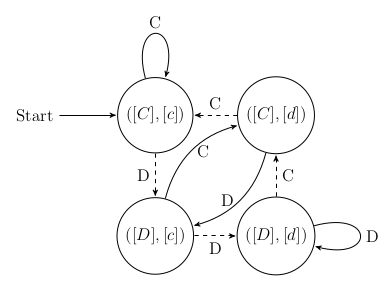
\includegraphics[width=0.9\linewidth]{img/titfortat.png}
\end{minipage}
\begin{minipage}{0.35\linewidth}
	\begin{itemize}
		\item Plain arrow if player 1 play tit-for-tat.
		\item Dashed arrow if player 1 play the opposite.
		\item Player 2 play tit-for-tat
	\end{itemize}
	\note{
		Make the graph on board if we play grim strategy
		
		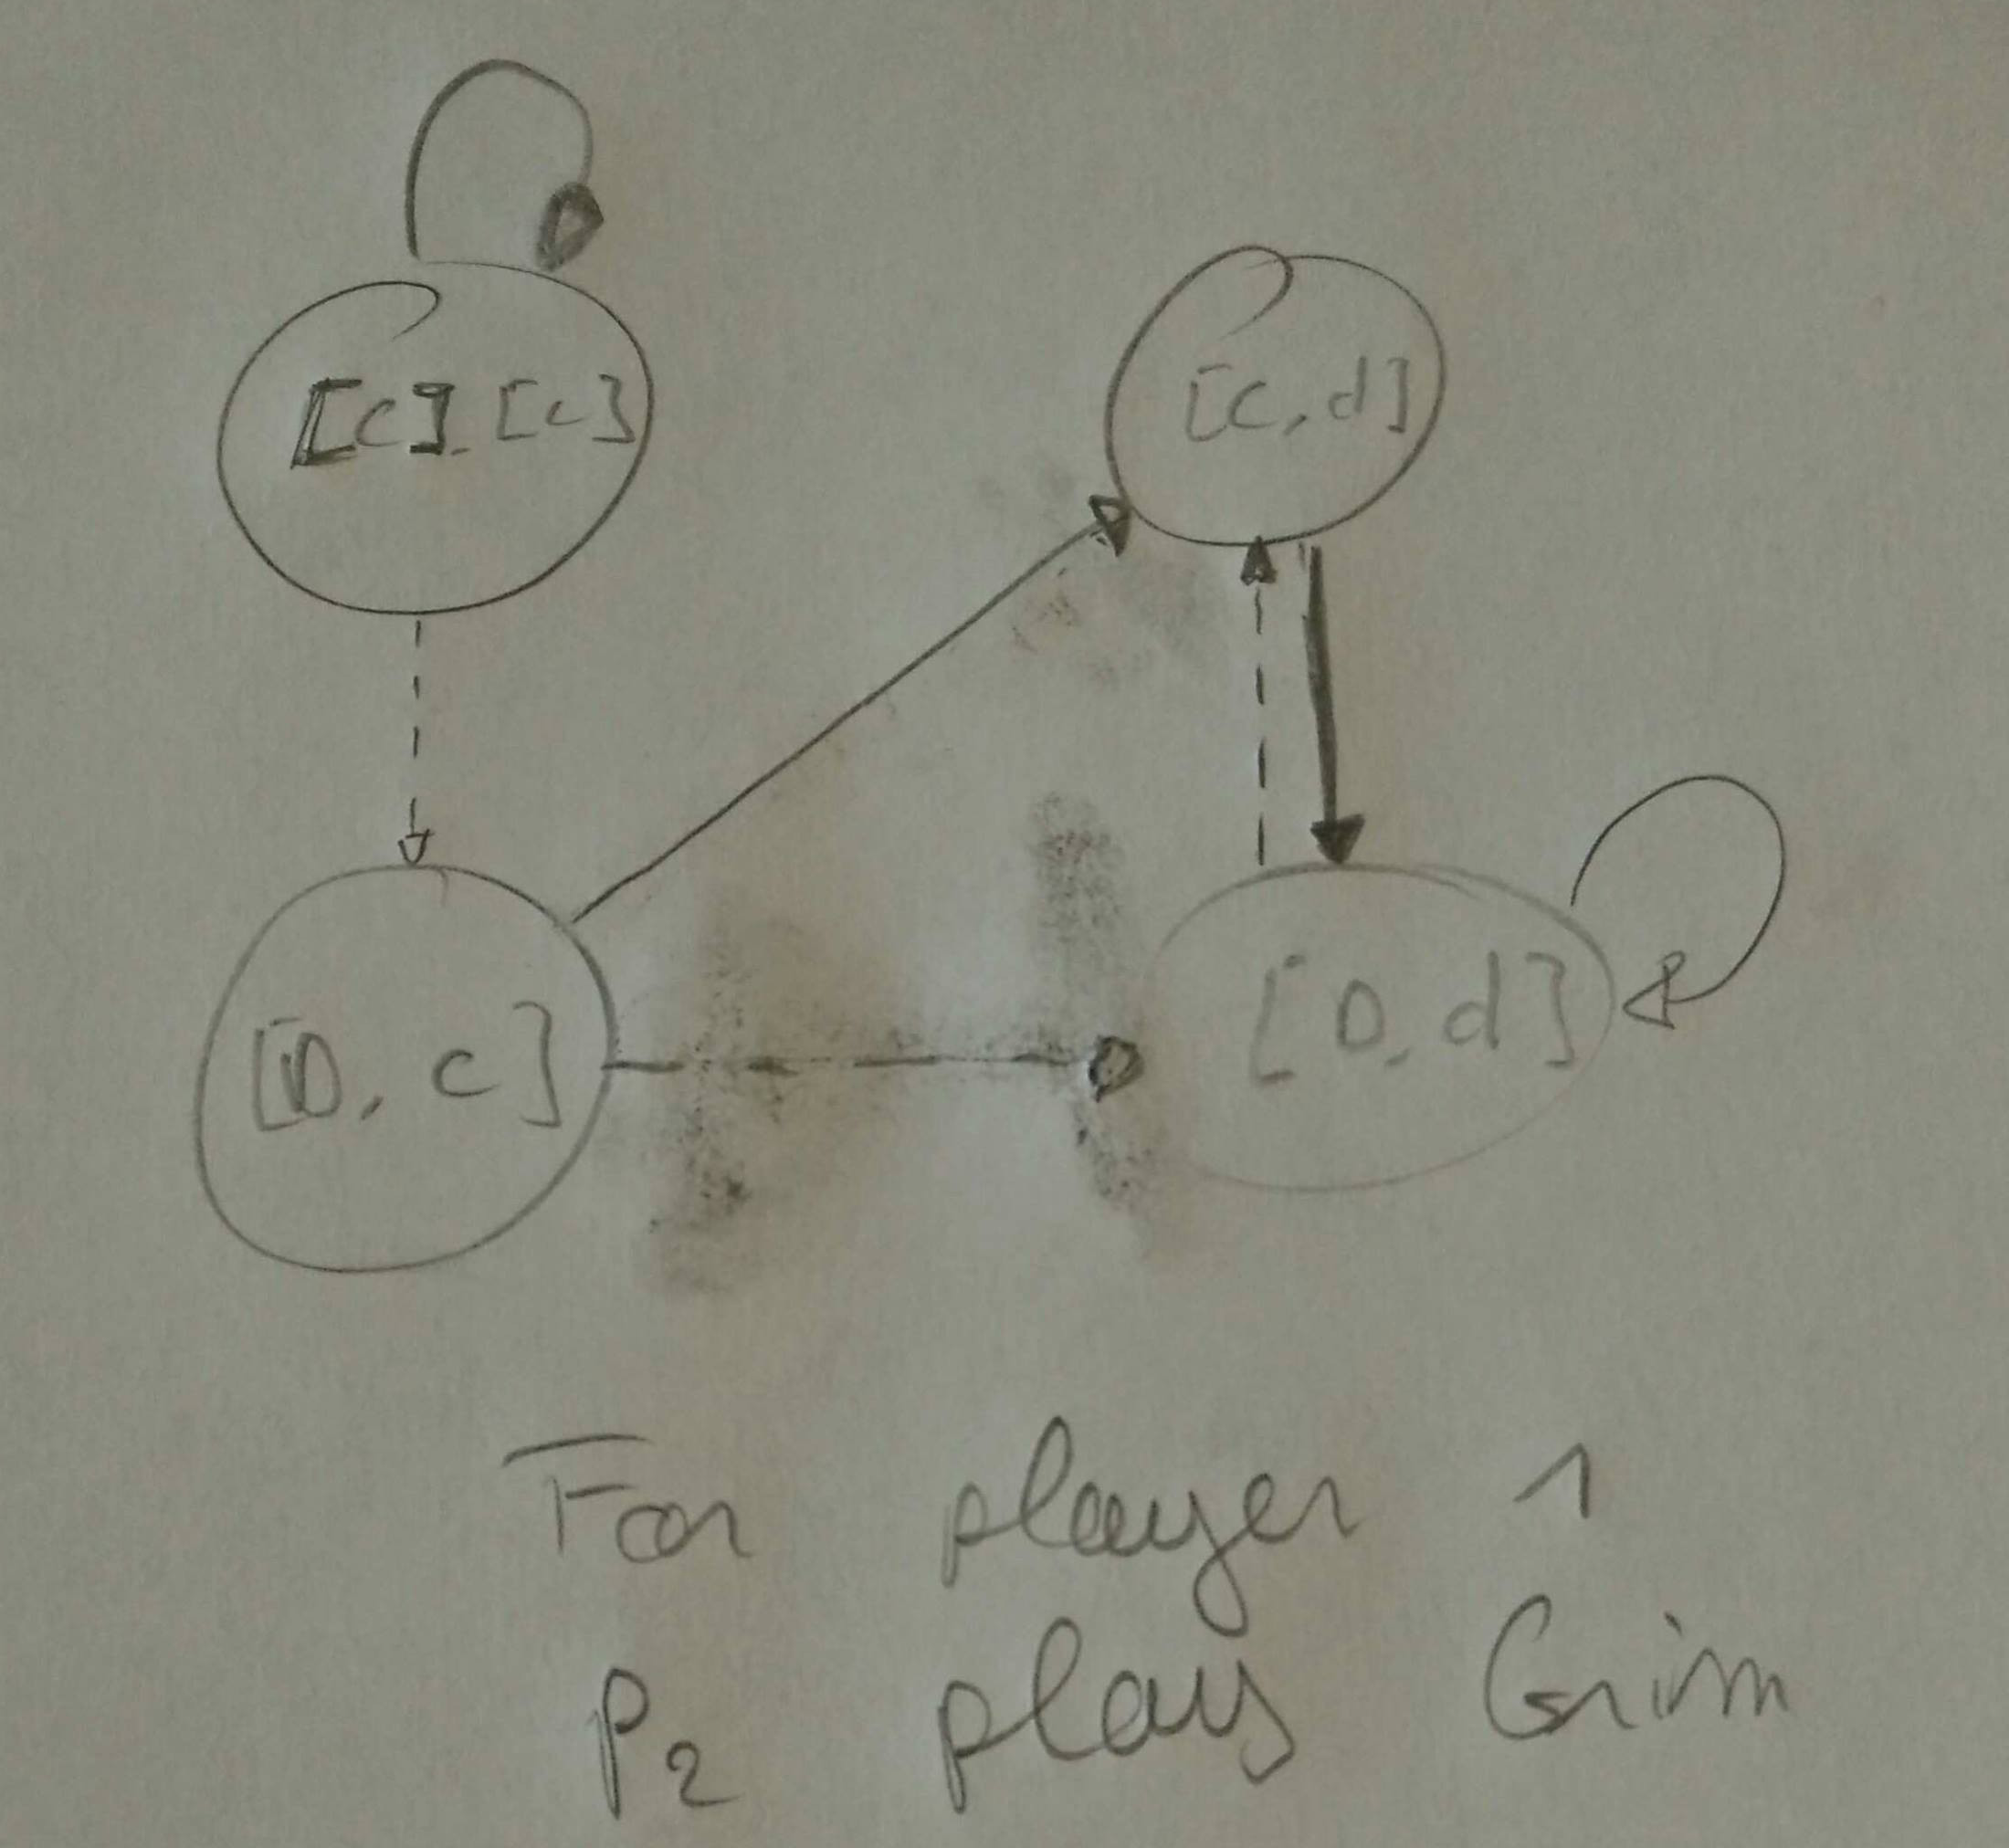
\includegraphics[width=0.5\linewidth]{img/ex_grim.jpg}	
	}
\end{minipage}

\end{frame}


\begin{frame}{Analyze the game}
Let's $\nu_i$ be the \textit{expected $\delta$-discounted average} of player $i$ when beginning from the state $\theta \in \Theta$ when everyone plays according to $\tau$.
\begin{small}
\begin{align*}
\nu_i(\theta, \tau) &=   \sum_{d_i \in D_i} \tau_i(d_i|\theta) \cdot Y_i(\tau, d_i, \nu_i, \theta, \delta)\\
&= \sum_{d_i \in D_i} \tau_i(d_i|\theta) \sum_{d_{-i} \in D_{-i}} \tau_{-i}(d_{-i} |\theta) \left( (1-\delta) u_i(d_i,\theta) + \delta \sum_{\hat{\theta}} p(\hat{\theta}|d,\theta) \nu_i(\hat{\theta},\tau) \right)  \\
&= \text{max}_{d_i \in D_i} Y_i(\tau, d_i, \nu_i, \theta, \delta)
\end{align*}
\end{small}
\begin{small}
\begin{align*}
Y_i(\tau, d_i, \nu_i, \theta, \delta) = \sum_{d_{-i} \in D_{-i}} \tau_{-i}(d_{-i} |\theta) \left( (1-\delta) u_i(d_i,\theta) + \delta \sum_{\hat{\theta}} p(\hat{\theta}|d,\theta) \nu_i(\hat{\theta},\tau) \right)
\end{align*}
\end{small}
This expression can be interpreted as the gain of player $i$ if he played the move $d_i$ once if at state $\theta$ everyone else follows $\tau$.
\end{frame}

\begin{frame}{Let's go back to the prisonner's dilema for a small example}
For a given $0 \leq \delta < 1$ we have the followin $\delta$-discounted payoff for player 1
	\begin{align*}
		\nu_1([C],[c]) &= (1-\delta) \cdot 1 + \delta \cdot \nu_1([C],[c])\\
		\nu_1([D],[c]) &= (1-\delta) \cdot -1 + \delta \cdot \nu_1([C],[c])\\
		\nu_1([C],[d]) &= (1-\delta) \cdot 2 + \delta \cdot \nu_1([C],[c])\\
		\nu_1([D],[d]) &= (1-\delta) \cdot 0 + \delta \cdot \nu_1([C],[c])
	\end{align*}
\pause
The solution are imediate:
\begin{align*}
	\nu_1([C],[c]) &= 1\\
	\nu_1([D],[c]) &= \frac{2\delta - 1}{1+\delta}\\
	\nu_1([C],[d]) &= \frac{2-\delta}{1+\delta}\\
	\nu_1([D],[d]) &= 0
\end{align*}
\end{frame}

\begin{frame}
	Then, to ensure that $\tau$ is an equilibrium of the repeated game, we must verify the equation $\nu_i(\theta) = \text{max}_{d_i \in D_i} Y_i(\tau, d_i, \nu_i, \theta, \delta)$. That is to ensure that the follwing inequalities are satisfied.
\begin{align*}
	\nu_1([C],[c]) &\geq (1-\delta)2 + \delta \nu_1([D],[c]) = \nu_1([C],[d]) \quad \text{Doing D instead of C}\\
	\nu_1([D],[c]) &\geq (1-\delta)0 + \delta \nu_1([D],[d]) = 0 \qquad \text{Doing D instead of C}\\
	\nu_1([C],[d]) &\geq (1-\delta)1 + \delta \nu_1([C],[c]) = 1 \qquad \text{Doing C instead of D}\\
	\nu_1([D],[d]) &\geq (1-\delta)(-1) + \delta \nu_1([C],[d]) = \nu_1([D],[c]) \quad \text{Doing C instead of D}
\end{align*}

\pause
\begin{itemize}
	\item For $\delta = 0.5$ : equilibrium reached
	\item For $\delta \leq 0.5$ : We play as for the non repetitive Prisoner's dilemma (search for immediate reward).
	\item For $\delta \geq 0.5$ : If we know that the other is going to play Tit-for-Tat, we should always play cooperate.
\end{itemize}
\end{frame}

\begin{frame}{A Taxonomy of Repeated Games Models}
    \begin{figure}
        \tikzstyle{mybox} = [draw=gray!20, fill=white, very thick,
        rectangle, rounded corners, inner sep=10pt, inner ysep=10pt]
        \tikzstyle{fancytitle} = [fill=gray, text=white, rounded corners]
        \scalebox{0.7}{
        \begin{tikzpicture}
            \node [mybox] at (0, 0) (gen-mod){%
                \begin{minipage}{0.50\textwidth}
                    \vspace{-0.25cm}
                    \[ \Gamma^r = (N, \Theta, (D_i, S_i, u_i)_{i\in N}, q, p) \]
                \end{minipage}
            };
            \node [inner sep=0pt] (gen-mod-img) at (-4.4, 0.5){%
                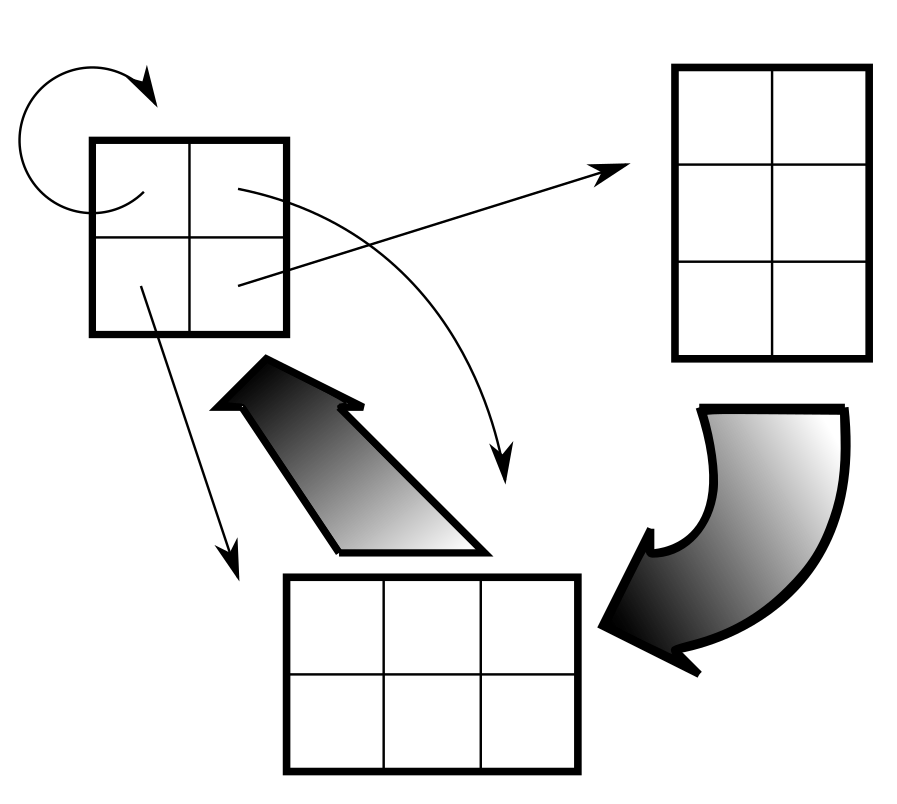
\includegraphics[width=0.25\textwidth]{img/stochastic.png}
            };
            
            \node [mybox] at (-4.5, -3) (mdp){%
                \begin{minipage}{0.40\textwidth}
                    {\color{green}Single-agent stochastic game}
                    \vspace{-0.25cm}
                    \[ |N| = 1. \]
                \end{minipage}
            };
            
            \node [mybox] at (0, -7.5) (state){%
                \begin{minipage}{\textwidth}
                    {\color{green}At every round, every player knows the
                    current state of nature $\theta \in \Theta$.} \\
                    Informally, for each player $i \in N$, there exists some
                    state $w(s_i) \in \Theta$ such that the signal $s_i$ can
                    never occur unless the current state is $w(s_i)$.
                \end{minipage}
            };
            
            \node [mybox, draw=black] at (4.5, -3.5) (std){%
                \begin{minipage}{0.60\textwidth}
                    \begin{itemize}
                        \item {\color{green}Only one possible state of
                        nature}
                        \[ |\Theta| = 1. \]
                        \item {\color{green}Players know all of each other's past
                        moves}
                        \[ S_i = \bigtimes_{j\in N-i} D_j. \]
                    \end{itemize}
                \end{minipage}
            };
            \node [inner sep=0pt] (gen-mod-img) at (7, -5.5){%
                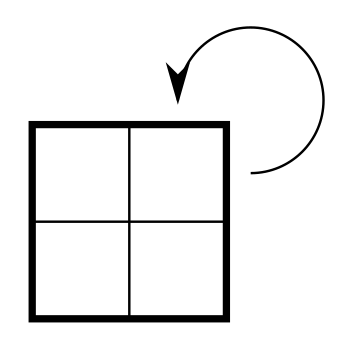
\includegraphics[width=0.20\textwidth]{img/std.png}
            };

            \node[fancytitle] at (gen-mod.north) {Stochastic Games (General Model)};
            \node[fancytitle] at (mdp.north) (mdp-title) {Markov Decision Processes};
            \node[fancytitle] at (state.north) (state-title) {Complete State Information};
            \node[fancytitle, fill=black] at (std.north) (std-title) {Standard Repeated Games};

            \draw[thick, -Latex] (gen-mod.west) -- (mdp-title.north);
            \draw[thick, -Latex] (gen-mod.south) -- (state-title.north);
            \draw[thick, -Latex] (gen-mod.east) -- (std-title.north);
        \end{tikzpicture}}
        \caption{A taxonomy of repeated game models.}
    \end{figure}
\end{frame}

\begin{frame}{Repeated game with standard information}
    \metroset{block=fill}
    \begin{block}{Definition}
        A \textbf{standard repeated game} is a repeated game in which there is only one state of
        possible state of nature
		$$|\Theta| = 1,$$
        the players know all of each other's past moves
        $$S_i = \bigtimes_{j \in N} D_j \quad \forall,$$
        and
		$$p(d,...,d,\theta | d, \theta) = 1 \quad \forall d \in D.$$
    \end{block}
\end{frame}


\begin{frame}{Example : the game of Chicken}
    \begin{exampleblock}{Example}
        Consider the game of Chicken in normal form
        \begin{table}
            \begin{tabular}{c|cc}
                & {\color{red}$a_2$}    & {\color{red}$b2$} \\
                \hline
                {\color{green}$a_1$}    & \payoff{4}{4}   & \payoff{1}{6} \\
                {\color{green}$b_1$}    & \payoff{6}{1}    & \payoff{-3}{-3} 
            \end{tabular}
            \caption{Game of Chicken in normal form}
        \end{table}
    
    \end{exampleblock}
    \note{
		Draw the normal form on the board    
		
		Explain the anecdote
    }
\end{frame}

\begin{frame}{Equilibrium of the single shot game}
\textbf{Analyze of the game}

\begin{itemize}
	\pause
	\item Nash equilibrium : (1,6) (6,1)
	\begin{itemize}
		\item Randomized equilibrium : $u_i = 0.5\cdot4 + 0.5 \cdot (6+1-3) = 3$
		\item Correlated equilibrium : $u_i = 0.5\cdot4 + 0.25 \cdot (6+1) =  3.75$
	\end{itemize}
	\pause
	\item Repetition of the game with standard information $$u_i = ??$$
\end{itemize}
	\pause
	Tit-for-tat is an equilibrium if $\delta \geq \frac{2}{3}$
\end{frame}

\note{
	Say that $(a_1,a_2)$ is not an sub-game perfect of the \textbf{one round} game because both players would want to play $b$

	\begin{itemize}
		\item \textbf{HYP}
			\begin{itemize}
				\item Infinitely repeated game with standard information
				\item Player 1 choose a $\delta$ between 0 and 1, what value of $\delta$
				\item Player 2 begin to be bold, and then be cautious at every round
			\end{itemize}
		\item Compute the $\delta$-discounted average payoff : $(1-\delta)(6+1\delta+\sum_{k=3}^\infty 4\delta^{k-1} ) = 6 - 5\delta + 3 \delta^2$
		\item $\delta$-discounted average if no deviation from tit-for-tat : $4 \geq 6 - 5\delta + 3 \delta^2$
		\item Tit-for-Tat is an equilibrium if $\delta \geq \frac{2}{3}$
	\end{itemize}
}

\begin{frame}{Going further with the Tit-for-Tat strategy in a standard information game}
	
	\textbf{Going further}
	\begin{itemize}
	\item What will be the $\delta$-discounted average payoff if both player decide to play Tit-for-Tat after player 2 deviation ?
	\pause
	
	\item What will be the $\delta$-discounted average payoff if p1 deviates from Tit-for-Tat after player 2 deviation. Then both play Tit-for-Tat.
	\pause
	\item What $\delta$ should we choose so that neither player can gain by being the first to deviate ?
	\end{itemize}
	\note{
	\textbf{Going further}
	\begin{itemize}
		\item If both player play Tit-for-tat after P2 deviation $(1-\delta)(1+6\delta+1\delta^2+6\delta^3+...) = \frac{1+6\delta}{1+\delta}$
		\item If P1 deviate after P2 deviation $(1-\delta)(1+4\delta+4\delta^2+4\delta^3+...) = 1+3\delta$
		\item $1+3\delta > \frac{1+6\delta}{1+\delta}$ when $\delta > \frac{2}{3}$
	\end{itemize}
	
	\textbf{Grim strategy}
	
	Only explain that such unforgiving punishment is not rational and extreme. We might be interested in finding other strategies.			
	}
\end{frame}

\begin{frame}{Finding mutual punishment strategies}
	\metroset{block=fill}
    \begin{block}{Mutual punishment strategy}
        For a player i, a {\color{green}mutual punishment strategy} can be :
        \begin{itemize}
        	\item On the first round : i plays $a_i$ \pause
        	\item If last round was $(a_1,a_2) \text{ or } (b_1,b_2)$, i plays $a_i$ \pause
        	\item If last round was $(a_1,b_2) \text{ or } (b_1,a_2)$, i plays $b_i$
        \end{itemize}
    \end{block}
    \textbf{\color{green}Interpretation}
    
    If both players follow the strategy, their expected payoff is 4. If one deviate, the other punish him until he participate himself in his own punishment.
    
    \textbf{\color{green}Is it a sub-game perfect equilibrium to follow the mutual punishment strategy?}
    
    \note{
		\textbf{If strategy call for $b_i$ but play $a_i$}
		
		Deviation is noob if $4+4\delta \geq 6 - 3 \delta \qquad \Rightarrow \delta \geq \frac{2}{7}$ not worth to deviate
		
		\textbf{If strategy call for $a_i$ but play $b_i$}
		
		Deviation is noob if $-3+4\delta \geq 1 - 3\delta \qquad \Rightarrow \delta	\geq \frac{4}{7}$ not worth to deviate
		
		    
    }
\end{frame}

\begin{frame}{Take home message \#6}
    \metroset{block=fill}

    \begin{block}{Take-home-message \#6}
        \vspace{0.2cm}
        \begin{columns}
            \begin{column}{0.65\textwidth}
                A \textbf{repeated game with standard information} is a repeated game where
                \begin{itemize}
                    \item there is {\color{green}only one possible state of nature}
                    \item the players {\color{green}know all of each other's past moves}
                \end{itemize}
            \end{column}
            \begin{column}{0.2\textwidth}
                \begin{center}
                    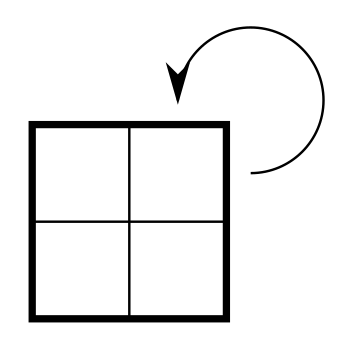
\includegraphics[width=0.7\linewidth]{img/std.png}
                \end{center}
            \end{column}
        \end{columns}

        \vspace{0.5cm}
        Depending on the value of the discount factor $\delta$, several strategies might constitute
        an equilibrium: \textit{tit-for-tat}, \textit{getting-even}, \textit{grim}, etc.
        However, these equilibria might not always be subgame perfect.
    \end{block}
\end{frame}

\begin{frame}[standout]
    Questions?
\end{frame}

\end{document}
